\chapter{Búsqueda en anchura (BFS)}
La BFS es similar a la DFS, en el sentido que explora todos los estados a los que se puede llegar a partir uno inicial.

Pero la diferencia es que esto los explora un orden diferente.

La DFS lo que hace es en un estado, explora totalmente lo que ofrezca una transición, y luego se regresa de esa exploración para ver la siguiente opción.

En cambio, la BFS lo que hace es llevar una lista de ``estados por explorar'' y procesarlos en orden. Para iniciar, revisamos todas las transiciones del estado inicial y los estados a los que nos lleven los agregamos en la lista.

Mostremos un diagrama del comportamiento de la BFS, en el diagrama los estados son representados por círculos y si han sido explorados los marcamos de gris, pero si están en la lista por explorar, los dejamos blancos. Las flechas representan las transiciones. Finalmente, los estados están enumerados en el orden que fueron alcanzados por la BFS.

\begin{center}
	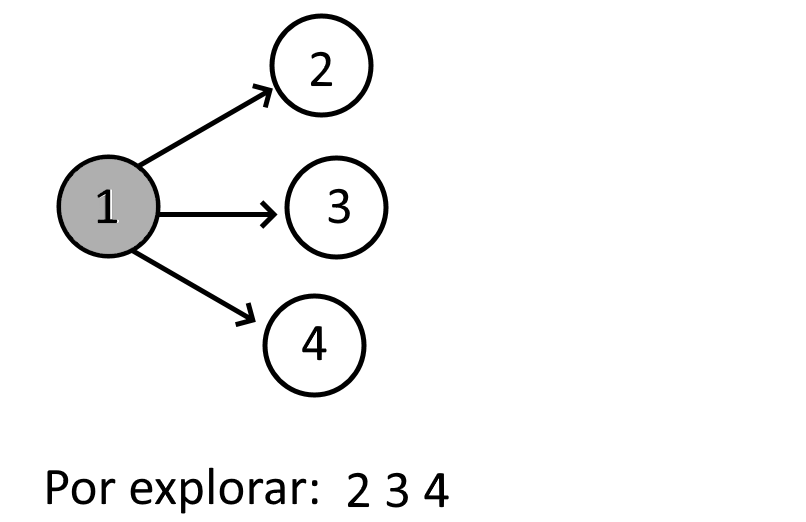
\includegraphics[scale=0.35]{bfs1}
\end{center}

Y luego para cada una de esos estados los exploramos también, es decir, expandimos las transiciones de esos estados y lo nuevo que encontremos lo ponemos en la lista de "estados por explorar". Importante: los visitamos en el orden que fueron agregados a la lista por explorar.

\begin{center}
	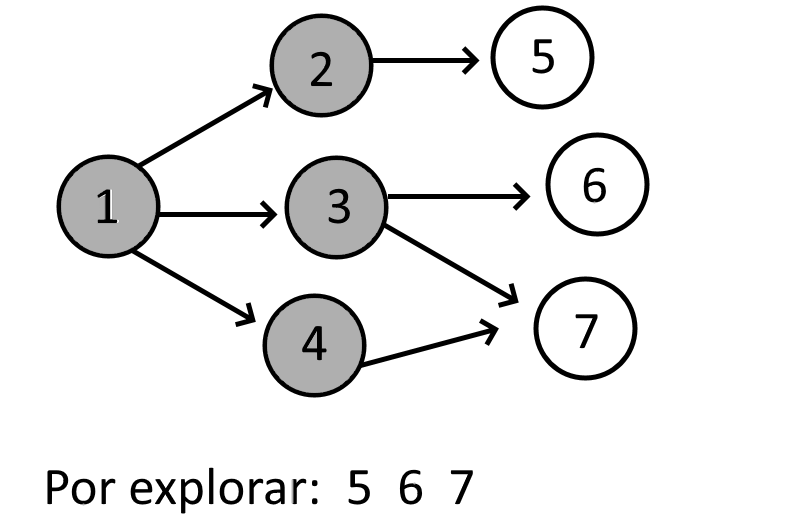
\includegraphics[scale=0.35]{bfs2}
\end{center}

De esta forma, comenzamos visitando todos los lugares alcanzables con una transición, luego dos transiciones, después tres, cuatro, cinco y  así sucesivamente.

Y precisamente, este orden en el que exploramos nos da una buena ventaja. A todo estado llegamos con la menor cantidad de transiciones posibles. Lo cual nos permite saber el mínimo número de transiciones necesarias para llegar e incluso lo podemos guardar en un arreglo o map para consultar después.

Para lograr este comportamiento, es importante ver que la lista por explorar se comporta de la siguiente forma: los estados son procesados en el mismo orden en el que entran, de forma que el primer estado en entrar a la lista es el primero en ser atendido. Este comportamiento es similar a la cola del cine, donde se atiende en el orden que llegas.

Para esto, podemos usar una estructura de datos de C++ llamada \verb|queue|, que significa cola en ingles. Si no sabes trabajar con ella, revisa la página \pageref{queue}.

Entonces, una BFS lo que hace es:

Tener una cola de la lista por explorar llamada \verb|explorar|, un arreglo de booleanos \verb|visitado| para marcar los estados que ya han sido descubiertos por la BFS y agregaremos un arreglo de enteros \verb|no_transiciones| para guardar cuantas transiciones requerimos para llegar a cada estado.

Comenzamos agregando a la lista por explorar el estado inicial con un \verb|no_transiciones| de \(0\). Luego, mientras todavía allá estados por explorar, lo procesaremos. Lo sacaremos de la pila al ya ser explorado y agregaremos a \verb|explorar| todos los estados que no hayan sido visitados alcanzables desde el estado que estamos procesando.

En código:

\begin{minipage}{\linewidth}
\begin{lstlisting}
bool visitado[];
int no_transiciones[];
void BFS(inicio) {
	queue<estados> explorar;
	cola.push(inicio);
	visitado[inicio]=true;
	no_transiciones[inicio]=0;
	while (explorar.empty()==false) {
		actual = explorar.front();
		cola.pop();
		if (actual es solucion) {
			registrar solucion actual;
			break; //opcional, si solo nos interesa una solucion
		}
		for (transiciones de actual) {
			if (!visitado[transicion]) {
				visitado[transicion]=true;
				no_transiciones[trancision]=
				no_transiciones[actual]+1;
				explorar.push(transicion);
			}
		}
	}
}
\end{lstlisting}
\end{minipage}

Como ya es de costumbre, veamos un ejemplo para entender esto.
\section{Ejemplo: Dos operaciones}
Javier tiene una calculadora un poco peculiar. Esta muestra un número \(x\) en pantalla y tiene dos botones.

\begin{plimits}
	\item El primer botón le suma \(a\) al valor de \(x\).
	\item El segundo botón le  suma \(\frac{x}{b}\) a \(x\), pero solo puede ser presionado cuando \(x\) sea un múltiplo de \(b\).
\end{plimits}

Ahora Javier se pregunta cuantas veces debe presionar un botón para que el valor \(x\) se convierta en \(y\).

\textbf{Entrada}\\
La entrada constará de cuatro enteros: \(x\), \(y\), \(a\) y \(b\). El valor inicial de la calculadora, el valor deseado, y el valor de \(a\) y \(b\) para los botones.

\textbf{Salida}\\
Imprime un entero que sea la cantidad de pulsaciones mínima para convertir \(x\) a \(y\). Si es imposible pasar de \(x\) a \(y\) imprime \(-1\).

\textbf{Ejemplo}\\
\begin{casebox3}
	\ecase{	1 20 4 5}{6}
	{	Presiona el primer botón, ahora tienes 5.\\		
		Usa el segundo, ahora vale 6.\\
		Pulsa el primer botón, obtienes 10.\\
		Utiliza el segundo para tener 12.\\
		Usa el primer botón, obtén 16.\\
		Termina con el primero, llegamos a 20.
	}
	\ecase{	1 32 3 2}{-1}
	{	Es imposible obtener 32.
	}
\end{casebox3}

\textbf{Límites}
\begin{plimits}
	\item \(1\leq x,y,a,b \leq 10^5\)
\end{plimits}

ENLACE: TODO

\subsection*{Solución}
Entonces, en este problema nos piden la mínima cantidad de operaciones para pasar de \(x\) al valor de \(y\).

Recordemos que la BFS es perfecta para esta situaciones, pues calcula la mínima cantidad de transiciones para pasar de un estado inicial a todos los demás, incluyendo \(y\).

Para esto haremos una BFS que use de estados el número de la calculadora y de transiciones los botones. Esta explorará todas las operaciones desde \(x\) hasta llegar a \(y\).

Esto se verá:

\begin{minipage}{\linewidth}
\begin{lstlisting}
	bool visitado[100005];
	int no_transiciones[100005];
	int bfs(int x, int y, int a, int b) {
		queue<int> cola;
		cola.push(x);
		visitado[x]=true;
		no_transiciones[x]=0;		
		while (cola.empty()==false) {
			int actual=cola.front();
			cola.pop();
			if (actual==y) {
				return no_transiciones[y];
			}	
			//Primer boton
			int siguiente = actual+a;
			if (vistado[siguiente]==false){
				visitado[siguiente]=true;
				no_transiciones[siguiente]=
				no_transiciones[actual]+1;
				cola.push(siguiente);
			}
			//Segundo boton
			siguiente = actual+actual/b;
			if (actual%b == 0 && vistado[siguiente]==false){
				visitado[siguiente]=true;
				no_transiciones[siguiente]=
				no_transiciones[actual]+1;
				cola.push(siguiente);
			}
		}
		return -1;
	}
\end{lstlisting}
\end{minipage}